\newcommand{\mola}[5]%Quanto menor for o valor 3,4 e 5 dado à função mais comprimida estará a mola%
{
%------------------------------------------------------------Pontos Importantes------------------------------------------------------------%
\coordinate (bola1) at (0,{#1});
\coordinate (bola2) at (0,{#2}); 
\coordinate (bola3) at (0,-6);
\coordinate (bola4) at (0,-10);
\coordinate (reticencias) at (0,-8);
%-------------------------------------------------------------Desenhar as Molas------------------------------------------------------------%
\tikzstyle{spring}=[thick,decorate,decoration={aspect=.5, segment length=#3, amplitude=2.5mm,coil}]
\tikzstyle{spring}=[thick,decorate,decoration={aspect=.5, segment length=#4, amplitude=2.5mm,coil}]
\draw [spring] (bola3) -- (bola2);
\tikzstyle{spring}=[thick,decorate,decoration={aspect=.5, segment length=#5, amplitude=2.5mm,coil}]
\draw [spring] (bola4) -- (bola3);
%-------------------------------------------------------------Desenhar as Bolas------------------------------------------------------------%
\shade [ball color =white] (bola2) circle (.5) node[draw=none,inner sep = 0,scale=2,text=black]{};
\shade [ball color =white] (bola3) circle (.5) node[draw=none,inner sep = 0,scale=2,text=black]{};
\shade [ball color =white] (bola4) circle (.5) node[draw=none,inner sep = 0,scale=2,text=black]{};
%----------------------------------------------------------Desenhar as Reticências--------------------------------------------------------%
\node[rectangle,fill=white, minimum width = 2cm, minimum height = 1.1cm] (r) at (reticencias) {};
\draw (reticencias) node[ultra thick,scale=1]{$\rotatebox{90}{$\cdots$}$} ;
}
\begin{minipage}{0.22\colwidth}
\resizebox{.2\colwidth}{!}{
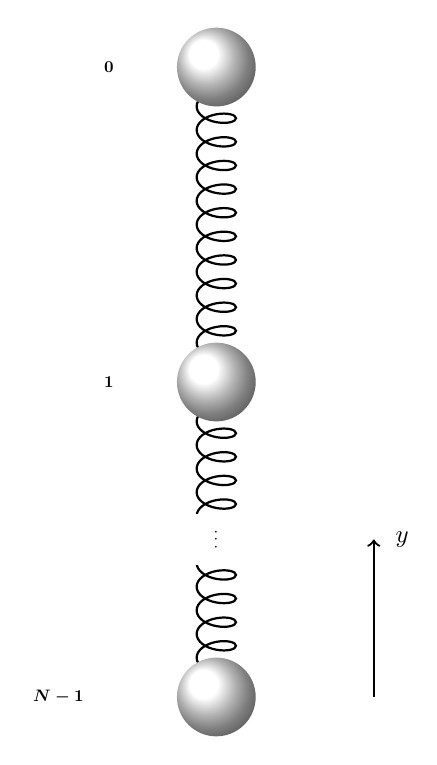
\begin{tikzpicture}[scale=1, every node/.style={scale=.6}]
\mola{2}{-2}{3mm}{3mm}{3mm}
\node[anchor=west] at (-1.5,-2) {\textbf{\boldmath$0$}};
\node[anchor=west] at (-1.5,-6) {\textbf{\boldmath$1$}};
\node[xshift=-1.5cm,anchor=west] at (-1.5,-10) {\textbf{\boldmath$N-1$}};
\draw[thick,->] (2,-10) -- (2,-8) node[draw=none,inner sep = 0,scale=1.5,xshift=.4cm,text=black]{$y$};
\end{tikzpicture}}
\end{minipage}
\begin{minipage}{0.7\colwidth}
Mola ideal com comprimento natural $L$ com constante elástica $K$, com $N$
partículas pontuais iguais com massa $m=M/N$, dispostas regularmente ao longo da
mola.
\begin{align*}
  l&=L/(N-1)&&\rightarrow\text{Comprimento de cada segmento}\\
  k&=K(N-1)&& \rightarrow\text{Constante elástica de cada segmento}\\
  m&=M/N    &&\rightarrow\text{Massa de cada partícula}
\end{align*}
Posições de equilíbrio iniciais:
\begin{equation*}
  y_i^0=y_0^0-i\left[l+\left(N-\frac{i+1}{2}\right)\frac{mg}{k}\right],\quad i>0
\end{equation*}
\end{minipage}\\[1cm]
Acelerações ($x_i=y_i-y_i^0$):
  \begin{align*}
    \ddot x_0 &=-Ng+\omega^2(x_1-x_0)\\
    \ddot x_i &= \omega^2(x_{i-1}-2x_i+x_{i+1}),\qquad i=1, \ldots, N-2\\
    \ddot x_{N-1} &=\omega^2(x_{N-2}-x_{N-1})
  \end{align*}
Este sistema de equações foi resolvido em Python/Numpy, usando a função
\texttt{solve\_ivp} da biblioteca SciPy.
